% Venue template is provisional.
% Replace IEEEtran if the final venue requires another template.
\documentclass[conference]{IEEEtran}

\usepackage{amsmath,amssymb}
\usepackage{booktabs,multirow,graphicx,xcolor}
\usepackage{hyperref}
\usepackage{cleveref}
\usepackage{siunitx}
\usepackage{tabularx,array}
\usepackage{tikz}
\usetikzlibrary{arrows.meta,positioning,shapes.geometric}

% Provisional title — subject to change
\title{Compositional Verification of PMP--IOPMP Isolation in RISC-V SoCs:\\
Reset Ordering, Initialization, and Transaction Invariants}

\author{
  Author One\thanks{TODO: affiliation} \\
  Author Two\thanks{TODO: affiliation}
}

% Auto-generated by scripts/analysis/generate_paper_artifacts.py
% Do not edit manually

\newcommand{\GitCommitMFiveTen}{681b2bd}
\newcommand{\GitCommitCurrent}{b0d66661b938ab55075fee650be0bfa55ec5249a}
\newcommand{\EvidenceFreezeDate}{2026-08-11}

\newcommand{\EvidenceSPZeroOneSim}{PASS}
\newcommand{\EvidenceSPZeroOneBmc}{BOUNDED\_EVIDENCE}
\newcommand{\EvidenceSPZeroOnePdr}{NOT\_RUN}
\newcommand{\EvidenceSPZeroOneClass}{BOUNDED\_EVIDENCE}

\newcommand{\EvidenceSPZeroTwoSim}{PASS}
\newcommand{\EvidenceSPZeroTwoBmc}{FORMAL\_PROOF}
\newcommand{\EvidenceSPZeroTwoPdr}{FORMAL\_PROOF}
\newcommand{\EvidenceSPZeroTwoClass}{FORMAL\_PROOF}

\newcommand{\EvidenceSPZeroThreeSim}{PASS}
\newcommand{\EvidenceSPZeroThreeBmc}{BOUNDED\_EVIDENCE}
\newcommand{\EvidenceSPZeroThreePdr}{NOT\_RUN}
\newcommand{\EvidenceSPZeroThreeClass}{BOUNDED\_EVIDENCE}

\newcommand{\EvidenceSPZeroFourSim}{PASS}
\newcommand{\EvidenceSPZeroFourBmc}{FORMAL\_PROOF}
\newcommand{\EvidenceSPZeroFourPdr}{FORMAL\_PROOF}
\newcommand{\EvidenceSPZeroFourClass}{FORMAL\_PROOF}

\newcommand{\EvidenceSPZeroFiveSim}{PASS}
\newcommand{\EvidenceSPZeroFiveBmc}{NOT\_RUN}
\newcommand{\EvidenceSPZeroFivePdr}{NOT\_RUN}
\newcommand{\EvidenceSPZeroFiveClass}{NOT\_RUN}

\newcommand{\EvidenceSPZeroSixSim}{PASS}
\newcommand{\EvidenceSPZeroSixBmc}{NOT\_RUN}
\newcommand{\EvidenceSPZeroSixPdr}{NOT\_RUN}
\newcommand{\EvidenceSPZeroSixClass}{NOT\_RUN}

\newcommand{\EvidenceSPZeroSevenSim}{PASS}
\newcommand{\EvidenceSPZeroSevenBmc}{NOT\_RUN}
\newcommand{\EvidenceSPZeroSevenPdr}{NOT\_RUN}
\newcommand{\EvidenceSPZeroSevenClass}{NOT\_RUN}

\newcommand{\EvidenceSPZeroEightRSTASim}{COUNTEREXAMPLE}
\newcommand{\EvidenceSPZeroEightRSTABmc}{RESET\_ASSUMPTION\_DEPENDENCY}
\newcommand{\EvidenceSPZeroEightRSTAPdr}{NOT\_RUN}
\newcommand{\EvidenceSPZeroEightRSTAClass}{RESET\_ASSUMPTION\_DEPENDENCY}

\newcommand{\EvidenceSPZeroEightRSTBSim}{PASS}
\newcommand{\EvidenceSPZeroEightRSTBBmc}{FORMAL\_PROOF}
\newcommand{\EvidenceSPZeroEightRSTBPdr}{FORMAL\_PROOF}
\newcommand{\EvidenceSPZeroEightRSTBClass}{FORMAL\_PROOF}

\newcommand{\EvidenceSPOneZeroSim}{PASS}
\newcommand{\EvidenceSPOneZeroBmc}{BOUNDED\_EVIDENCE}
\newcommand{\EvidenceSPOneZeroPdr}{NOT\_RUN}
\newcommand{\EvidenceSPOneZeroClass}{BOUNDED\_EVIDENCE}

\newcommand{\EvidenceSPOneOneSim}{NOT\_RUN}
\newcommand{\EvidenceSPOneOneBmc}{FORMAL\_HARNESS\_BUG}
\newcommand{\EvidenceSPOneOnePdr}{NOT\_RUN}
\newcommand{\EvidenceSPOneOneClass}{FORMAL\_HARNESS\_BUG}

\newcommand{\EvidenceSPOneThreeSim}{NOT\_RUN}
\newcommand{\EvidenceSPOneThreeBmc}{COUNTEREXAMPLE}
\newcommand{\EvidenceSPOneThreePdr}{FORMAL\_PROOF}
\newcommand{\EvidenceSPOneThreeClass}{COUNTEREXAMPLE}

\newcommand{\EvidenceSPBZeroOneSim}{NOT\_RUN}
\newcommand{\EvidenceSPBZeroOneBmc}{BOUNDED\_EVIDENCE}
\newcommand{\EvidenceSPBZeroOnePdr}{NOT\_RUN}
\newcommand{\EvidenceSPBZeroOneClass}{BOUNDED\_EVIDENCE}

\newcommand{\EvidenceMFiveSevenFPZeroFourFIXZeroSim}{COUNTEREXAMPLE}
\newcommand{\EvidenceMFiveSevenFPZeroFourFIXZeroBmc}{EXPECTED\_PRE\_FIX\_COUNTEREXAMPLE}
\newcommand{\EvidenceMFiveSevenFPZeroFourFIXZeroPdr}{NOT\_RUN}
\newcommand{\EvidenceMFiveSevenFPZeroFourFIXZeroClass}{EXPECTED\_PRE\_FIX\_COUNTEREXAMPLE}

\newcommand{\EvidenceMFiveSevenFPZeroFourFIXTwoSim}{BOUNDED\_PASS}
\newcommand{\EvidenceMFiveSevenFPZeroFourFIXTwoBmc}{BOUNDED\_PASS}
\newcommand{\EvidenceMFiveSevenFPZeroFourFIXTwoPdr}{FAIL (raw; see classification: BOUNDED\_EVIDENCE)}
\newcommand{\EvidenceMFiveSevenFPZeroFourFIXTwoClass}{BOUNDED\_EVIDENCE}


% Auto-generated provenance
\newcommand{\ProvenanceCommit}{b0d66661b938ab55075fee650be0bfa55ec5249a}
\newcommand{\ProvenanceScriptHash}{226708a3ff15}
\newcommand{\ProvenanceGenerated}{2026-08-11T05:25:27.524522+00:00}
\newcommand{\ProvenanceGuaranteeCsv}{results/tables/m510\_guarantee\_matrix.csv}
\newcommand{\ProvenanceSensitivityCsv}{results/tables/m510\_assumption\_sensitivity.csv}


\begin{document}
\maketitle

% TODO(PROSE): Final abstract not written in M6.
% Structured skeleton only.

\begin{abstract}
\textbf{Problem:} CPU-side PMP and DMA-side IOPMP-style mechanisms protect different transaction origins in RISC-V SoCs.

\textbf{Research question:} Whether local access-control correctness composes into an end-to-end protected-memory isolation guarantee.

\textbf{Method:} RTL simulation, randomized tests, bounded model checking, and induction/PDR where applicable, with assumption sensitivity.

\textbf{Verified result:} Selected normal-operation CPU/DMA access-control properties (e.g., SP-02, SP-04) are formally established under documented assumptions.

\textbf{Compositional result:} Under RST-A fail-open initialization, an unsafe early-DMA protected-memory state before \texttt{secure\_ready} is reachable (RESET\_ASSUMPTION\_DEPENDENCY). Under RST-B fail-closed defaults, the corresponding state is unreachable (FORMAL\_PROOF via k-induction).

\textbf{Conclusion:} Compositional isolation depends on initialization, reset ordering, requester identity, and transaction-admission invariants---not local rules alone.

% EVIDENCE: results/m510/m510_summary.md
\end{abstract}

% SOURCE: results/m510/m510_summary.md
\section{Introduction}
\label{sec:intro}

% VERIFIED FACT: PMP mediates CPU-originated accesses; IOPMP-style logic mediates DMA/I/O.
% TODO(PROSE): Motivation paragraph.

% VERIFIED FACT: Local SP-02/SP-04 proofs do not automatically imply compositional guarantees.
% TODO(PROSE): Research gap.

\subsection{Research Question}
% TODO(PROSE): End-to-end compositional isolation under reset/initialization/admission.

\subsection{Contributions (PROVISIONAL --- pending literature review)}
\begin{itemize}
  \item \textbf{C1:} Compositional security model spanning PMP, IOPMP-style mediation, requester identity, admission, protected memory, reset state. % EVIDENCE: docs/security_properties.md
  \item \textbf{C2:} Reproducible workflow: simulation + BMC + induction where applicable. % EVIDENCE: Makefile m510
  \item \textbf{C3:} Reset-ordering characterization: RST-A reachable unsafe state vs RST-B excluded. % EVIDENCE: SP-08
  \item \textbf{C4:} Assumption-sensitivity analysis (initialization, identity, transaction invariants). % EVIDENCE: m510_assumption_sensitivity.csv
\end{itemize}

% Do not claim ``first'' without literature support.

\section{Background}
\label{sec:background}

% VERIFIED: RISC-V PMP restricts CPU accesses; project uses abstract CPU master (not Ibex).
% TODO(PROSE): PMP overview.

% VERIFIED: Research IOPMP-style model for DMA; not claimed fully standards-compliant unless demonstrated.
% TODO(PROSE): IOPMP / DMA mediation.

% VERIFIED: secure_ready = pmp_enable && iopmp_enable && rule0_valid
% EVIDENCE: rtl/soc/security_config.v

\section{Threat Model}
\label{sec:threat}

% SOURCE: docs/formal_assumptions.md, docs/m59_axi_environment_contract.md
% VERIFIED: Trusted configuration (FA-01: !cfg_write in baseline formal).
% VERIFIED: Authentic requester ID unless experiment models corruption (FA-02).
% TODO(PROSE): Adversary capabilities within modeled scope.

% Figure in Section~\ref{sec:system} (system model).

\section{System Model}
\label{sec:system}

% VERIFIED: Abstract CPU master + DMA master + interconnect + protected SRAM.
% VERIFIED: security_config provides secure_ready gating.
% LIMITATION: Not a complete RISC-V core or production SoC.

% Architecture figure — abstract research model (not Ibex)
\begin{figure}[t]
\centering
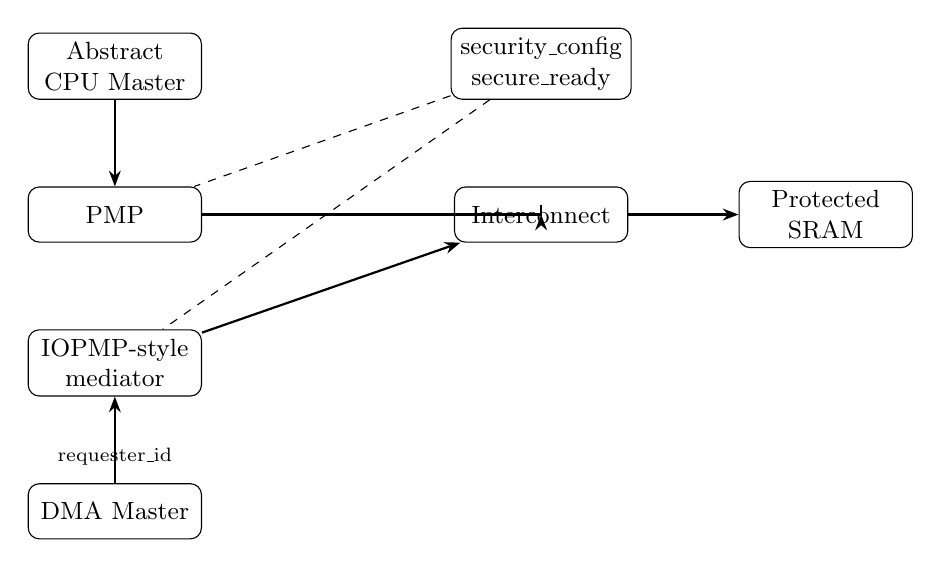
\begin{tikzpicture}[
  node distance=1.1cm and 1.4cm,
  box/.style={draw, rounded corners, minimum width=2.2cm, minimum height=0.7cm, align=center, font=\small},
  arr/.style={-{Stealth[length=2mm]}, thick}
]
  \node[box] (cpu) {Abstract\\CPU Master};
  \node[box, below=of cpu] (pmp) {PMP};
  \node[box, right=3.2cm of pmp] (ic) {Interconnect};
  \node[box, right=of ic] (sram) {Protected\\SRAM};
  \node[box, below=of pmp] (iopmp) {IOPMP-style\\mediator};
  \node[box, below=of iopmp] (dma) {DMA Master};
  \node[box, above=of ic] (sec) {security\_config\\secure\_ready};

  \draw[arr] (cpu) -- (pmp);
  \draw[arr] (pmp) -| (ic);
  \draw[arr] (dma) -- (iopmp);
  \draw[arr] (iopmp) -- (ic);
  \draw[arr] (ic) -- (sram);
  \draw[dashed] (sec) -- (iopmp);
  \draw[dashed] (sec) -- (pmp);
  \node[font=\scriptsize, above=0.1cm of dma] {requester\_id};
\end{tikzpicture}
\caption{Abstract compositional model: CPU path via PMP; DMA path via IOPMP-style mediation. \texttt{secure\_ready} gates secure operation.}
\label{fig:architecture}
\end{figure}


\section{Security Properties}
\label{sec:properties}

% SOURCE: docs/security_properties.md, results/tables/m510_guarantee_matrix.csv

\subsection{Representative Properties}
\begin{itemize}
  \item \textbf{SP-02:} Unauthorized CPU writes must not modify protected memory.
  \item \textbf{SP-04:} Unauthorized DMA writes must not modify protected memory.
  \item \textbf{SP-06:} Decisions must match DMA requester identity (simulation evidence).
  \item \textbf{SP-08:} Reset safety --- no unintentional protected accessibility interval.
  \item \textbf{M57-FP-04:} AXI write beat bound to authorized transaction context (full-RTL path).
\end{itemize}

% Auto-generated property summary (main paper subset)
\begin{table}[t]
\centering
\caption{Representative security properties: simulation vs formal methods. PDR column shows raw engine status where applicable; scientific classification is separate.}
\label{tab:property-summary}
\small
\begin{tabularx}{\linewidth}{@{}lXXXXl@{}}
\toprule
Property & Sim & BMC & PDR/Induct. & Scientific status \\
\midrule
SP-02 & PASS & FORMAL\_PROOF & FORMAL\_PROOF & FORMAL\_PROOF \\
SP-04 & PASS & FORMAL\_PROOF & FORMAL\_PROOF & FORMAL\_PROOF \\
SP-06 & PASS & NOT\_RUN & NOT\_RUN & NOT\_RUN \\
SP-08-RST-A & COUNTEREXAMPLE & RESET\_ASSUMPTION\_DEPENDENCY & NOT\_RUN & RESET\_ASSUMPTION\_DEPENDENCY \\
SP-08-RST-B & PASS & FORMAL\_PROOF & FORMAL\_PROOF & FORMAL\_PROOF \\
M57-FP-04-FIX2 & BOUNDED\_PASS & BOUNDED\_PASS & FAIL (raw; see classification: BOUNDED\_EVIDENCE) & BOUNDED\_EVIDENCE \\
\bottomrule
\end{tabularx}
\end{table}


\section{Verification Methodology}
\label{sec:method}

\begin{figure}[t]
\centering
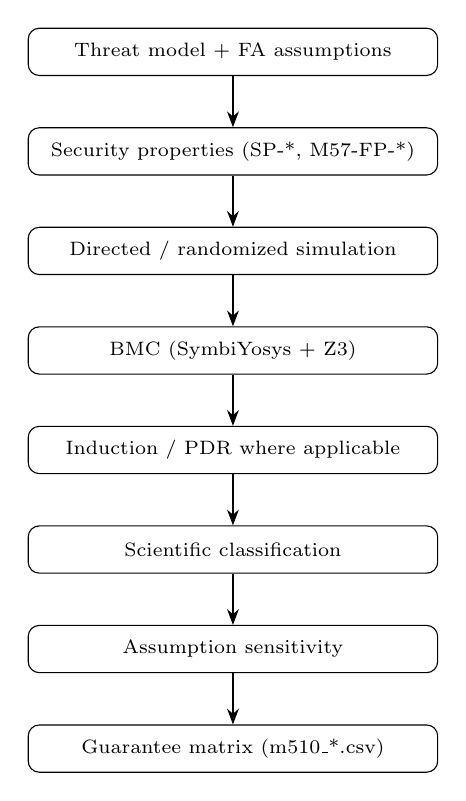
\begin{tikzpicture}[
  node distance=0.65cm,
  box/.style={draw, rounded corners, minimum width=5.2cm, minimum height=0.6cm, align=center, font=\scriptsize},
  arr/.style={-{Stealth[length=2mm]}}
]
  \node[box] (tm) {Threat model + FA assumptions};
  \node[box, below=of tm] (sp) {Security properties (SP-*, M57-FP-*)};
  \node[box, below=of sp] (sim) {Directed / randomized simulation};
  \node[box, below=of sim] (bmc) {BMC (SymbiYosys + Z3)};
  \node[box, below=of bmc] (ind) {Induction / PDR where applicable};
  \node[box, below=of ind] (cls) {Scientific classification};
  \node[box, below=of cls] (sen) {Assumption sensitivity};
  \node[box, below=of sen] (mat) {Guarantee matrix (m510\_*.csv)};
  \foreach \a/\b in {tm/sp,sp/sim,sim/bmc,bmc/ind,ind/cls,cls/sen,sen/mat} \draw[arr] (\a)--(\b);
\end{tikzpicture}
\caption{Verification workflow emphasizing classification distinct from raw tool status.}
\label{fig:workflow}
\end{figure}


% VERIFIED: Directed + randomized simulation (M1/M2), SymbiYosys BMC/induction, Verilator assertions (M57).
% VERIFIED: Scientific classification distinct from raw engine status.
% EVIDENCE: docs/m510_inconclusive_closure.md

\section{Experimental and Formal Results}
\label{sec:results}

% SOURCE: results/tables/m510_guarantee_matrix.csv

\subsection{Local Access Control}
% VERIFIED: SP-02 FORMAL_PROOF (k-induction); SP-04 FORMAL_PROOF.
% EVIDENCE: results/formal/sp02_pmp_prove, sp04_iopmp_prove

\subsection{Reset Ordering (SP-08)}
% Auto-generated reset model comparison
\begin{table}[t]
\centering
\caption{RST-A (fail-open) vs RST-B (fail-closed) under SP-08. RST-A counterexample is classified as reset-assumption dependency, not a vulnerability.}
\label{tab:reset-comparison}
\begin{tabular}{@{}lllll@{}}
\toprule
Model & Default & DMA before \texttt{secure\_ready} & Formal & Classification \\
\midrule
RST-A & fail-open & reachable (CE) & RESET\_ASSUMPTION\_DEPENDENCY & RESET\_ASSUMPTION\_DEPENDENCY \\
RST-B & fail-closed & unreachable & k-induction proof & FORMAL\_PROOF \\
\bottomrule
\end{tabular}
\end{table}

\begin{figure}[t]
\centering
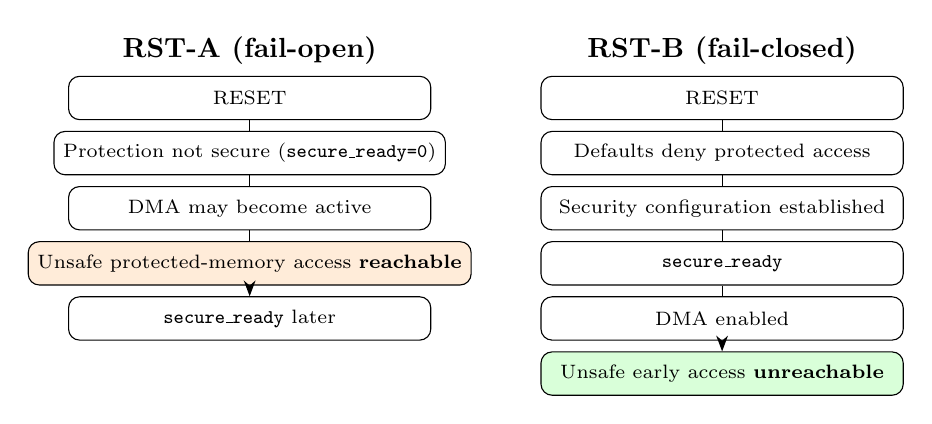
\begin{tikzpicture}[
  node distance=0.55cm,
  flowstep/.style={draw, rounded corners, minimum width=4.6cm, minimum height=0.55cm, align=center, font=\scriptsize},
  arr/.style={-{Stealth[length=2mm]}}
]
  \node[font=\bfseries] at (0,2.8) {RST-A (fail-open)};
  \node[flowstep] (a1) at (0,2.2) {RESET};
  \node[flowstep] (a2) at (0,1.5) {Protection not secure (\texttt{secure\_ready=0})};
  \node[flowstep] (a3) at (0,0.8) {DMA may become active};
  \node[flowstep, fill=orange!15] (a4) at (0,0.1) {Unsafe protected-memory access \textbf{reachable}};
  \node[flowstep] (a5) at (0,-0.6) {\texttt{secure\_ready} later};
  \draw[arr] (a1)--(a2)--(a3)--(a4)--(a5);

  \node[font=\bfseries] at (6,2.8) {RST-B (fail-closed)};
  \node[flowstep] (b1) at (6,2.2) {RESET};
  \node[flowstep] (b2) at (6,1.5) {Defaults deny protected access};
  \node[flowstep] (b3) at (6,0.8) {Security configuration established};
  \node[flowstep] (b4) at (6,0.1) {\texttt{secure\_ready}};
  \node[flowstep] (b5) at (6,-0.6) {DMA enabled};
  \node[flowstep, fill=green!15] (b6) at (6,-1.3) {Unsafe early access \textbf{unreachable}};
  \draw[arr] (b1)--(b2)--(b3)--(b4)--(b5)--(b6);
\end{tikzpicture}
\caption{Reset-ordering contrast for SP-08. RST-A CE is RESET\_ASSUMPTION\_DEPENDENCY, not labeled a vulnerability.}
\label{fig:reset-ordering}
\end{figure}


% VERIFIED RST-A: CE step 1, RESET_ASSUMPTION_DEPENDENCY — NOT a vulnerability claim.
% VERIFIED RST-B: k-induction proof (SymbiYosys smtbmc z3), FORMAL_PROOF.
% EVIDENCE: results/formal/counterexamples/SP-08/, sp08_rstb_prove/logfile.txt

\subsection{Requester Identity}
% VERIFIED: SP-06 simulation PASS (security_matrix.csv M2-RID-*).
% LIMITATION: No standalone formal proof row for SP-06 in m510 matrix.

\subsection{Write-Path Binding (M57-FP-04)}
% VERIFIED FIX-2: simulation BOUNDED_PASS; BMC ENV-4 BOUNDED_PASS; PDR raw FAIL.
% SCIENTIFIC: BOUNDED_EVIDENCE — not unbounded proof.
% VERIFIED M5.8 CE: HARNESS_ARTIFACT (closed M5.9).

% Auto-generated claims-to-evidence (main paper subset)
\begin{table*}[t]
\centering
\caption{Claims-to-evidence mapping (subset). Full register: \texttt{results/m6/claims\_evidence.csv}.}
\label{tab:claims-evidence}
\footnotesize
\begin{tabularx}{\textwidth}{@{}lXll@{}}
\toprule
ID & Claim & Status & Evidence \\
\midrule
CL-01 & CPU unauthorized protected-memory writes blocked by modeled PMP under stated ass... & FORMAL\_PROOF & results/tables/m510\_guarantee\_matrix.csv \\
CL-02 & Unauthorized DMA protected-memory writes blocked by modeled IOPMP under stated a... & FORMAL\_PROOF & results/tables/m510\_guarantee\_matrix.csv \\
CL-03 & Fail-open reset model permits reachable early-DMA protected-memory state before ... & RESET\_ASSUMPTION\_DEPENDENCY & results/formal/counterexamples/SP-08/ \\
CL-04 & Fail-closed reset model excludes corresponding unsafe state under formal model a... & FORMAL\_PROOF & results/formal/sp08\_rstb\_prove/logfile.t \\
CL-05 & Requester identity participates in access-control decisions... & PASS (simulation) & results/tables/security\_matrix.csv \\
CL-06 & M57-FP-04 write-binding on repaired RTL has bounded evidence, not unbounded proo... & BOUNDED\_EVIDENCE & results/tables/m510\_guarantee\_matrix.csv \\
\bottomrule
\end{tabularx}
\end{table*}

% Auto-generated assumption sensitivity (main paper subset)
\begin{table}[t]
\centering
\caption{Assumption sensitivity (subset). Full matrix in appendix.}
\label{tab:assumption-sensitivity}
\small
\begin{tabularx}{\linewidth}{@{}lXXl@{}}
\toprule
Assumption & Baseline & If removed/weakened & Classification \\
\midrule
M59-FA-04 & ENV-4 FIX-2 primary pass & CE returns step 5 & reset/anyinit artifact \\
M59-FA-11 & ENV-4 FIX-2 primary pass & FIX-2 primary CE & master quiescence required \\
M59-FA-10 & ENV-4 FIX-2 primary pass & txn\_active anyinit CE & observer consistency \\
M59-FA-07 & ENV-4 FIX-2 primary pass & spurious ini\_w at reset edge & post-reset idle \\
M59-FA-01 & ENV-4 FIX-2 primary pass & illegal AW morphing & protocol-required \\
M59-FA-05 & ENV-4 FIX-2 primary pass & W without txn CE & implementation sequencing \\
\bottomrule
\end{tabularx}
\end{table}


\section{Discussion}
\label{sec:discussion}

% VERIFIED STATEMENT (scoped):
% Compositional PMP--IOPMP isolation depends on initialization, reset ordering,
% requester identity, and transaction-admission invariants.
% EVIDENCE: results/m510/m510_summary.md section 13

% TODO(PROSE): Interpret RST-A as compositional assumption dependency, not exploit.

% TODO(PROSE): Contrast bounded evidence (M57-FP-04) vs formal proof (SP-02/04/08-RST-B).

\section{Related Work}
\label{sec:related}

% TODO(LITERATURE): Do not fabricate citations.
% Categories for future review:
% - PMP / ePMP formal verification
% - IOPMP / DMA isolation
% - SoC bus firewalls
% - RISC-V TEEs / enclaves
% - Compositional SoC security
% - Reset / lifecycle security
% - OpenTitan
% - Formal hardware security

% Local resource: riscv_key_isolation_literature_usage_guide.md
% Candidate list: results/m6/nearest_work_candidates.csv (metadata only; not auto-cited)

% PROVISIONAL: Novelty comparison deferred until verified bibliography exists.

\section{Limitations}
\label{sec:limitations}

% SOURCE: results/m6/limitations.md
% Auto-included from results/m6/limitations.md (M6)
\begin{itemize}
  \item \textbf{Abstract CPU master} --- not a complete RISC-V core (e.g., not Ibex).
  \item \textbf{Research IOPMP model} --- not claimed fully standards-compliant RISC-V IOPMP unless explicitly demonstrated.
  \item \textbf{No FPGA or ASIC/silicon validation.}
  \item \textbf{No claim of complete RISC-V SoC security.}
  \item \textbf{Bounded evidence} for some properties (e.g., M57-FP-04 FIX-2); PDR raw FAIL is not a confirmed violation.
  \item \textbf{SP-11} formal harness: PREUNSAT (FORMAL\_HARNESS\_BUG).
  \item \textbf{Yices unavailable} --- PDR witness replay TOOLCHAIN\_LIMITATION.
  \item \textbf{RST-A counterexample} is RESET\_ASSUMPTION\_DEPENDENCY at model level, not a named-product vulnerability.
  \item \textbf{PPA} (area, power, timing) not evaluated in current artifacts.
  \item Conclusions hold only under documented formal assumptions (FA-*, M59-FA-*).
\end{itemize}


\section{Reproducibility}
\label{sec:repro}

% VERIFIED commands:
\begin{itemize}
  \item \texttt{make m510-matrix} --- regenerate guarantee tables
  \item \texttt{make m510} --- full M5.10 reproduction suite
  \item \texttt{make paper} --- regenerate artifacts and compile PDF
\end{itemize}

% Provenance: commit \ProvenanceCommit{}, generated \ProvenanceGenerated{}.
% Branch: \texttt{m6-publication-freeze}. M5.10 checkpoint tag: \texttt{checkpoint-m510-complete} on \GitCommitMFiveTen{}.

% Toolchain: Yosys 0.68+ (read\_slang), SymbiYosys, Z3 5.0.0, Verilator 5.050.
% Yices witness replay: unavailable (TOOLCHAIN\_LIMITATION).

See Appendix~\ref{app:repro} for artifact paths and formal-engine commands.

\section{Conclusion}
\label{sec:conclusion}

% TODO(PROSE): Summarize scoped compositional dependency findings.
% VERIFIED: Local SP-02/SP-04 proofs + RST-A/B contrast + assumption sensitivity.
% Do not overgeneralize to all RISC-V systems.


\bibliographystyle{IEEEtran}
\bibliography{references}

\appendices
\section{Full Property Matrix}
\label{app:full-matrix}

% SOURCE: results/tables/m510_guarantee_matrix.csv
\footnotesize
\begin{tabular}{@{}lllll@{}}
\toprule
Property & Sim & BMC & PDR & Classification \\
\midrule
SP-01 & PASS & BOUNDED\_EVIDENCE & NOT\_RUN & BOUNDED\_EVIDENCE \\
SP-02 & PASS & FORMAL\_PROOF & FORMAL\_PROOF & FORMAL\_PROOF \\
SP-03 & PASS & BOUNDED\_EVIDENCE & NOT\_RUN & BOUNDED\_EVIDENCE \\
SP-04 & PASS & FORMAL\_PROOF & FORMAL\_PROOF & FORMAL\_PROOF \\
SP-08-RST-A & COUNTEREXAMPLE & RESET\_ASSUMPTION\_DEP. & NOT\_RUN & RESET\_ASSUMPTION\_DEPENDENCY \\
SP-08-RST-B & PASS & FORMAL\_PROOF & FORMAL\_PROOF & FORMAL\_PROOF \\
M57-FP-04-FIX2 & BOUNDED\_PASS & BOUNDED\_PASS & FAIL (raw) & BOUNDED\_EVIDENCE \\
\bottomrule
\end{tabular}

% Full CSV: repository results/tables/m510\_guarantee\_matrix.csv

\section{Formal Assumptions}
\label{app:assumptions}

% SOURCE: docs/formal_assumptions.md, docs/m59_formal_assumptions.md
\begin{itemize}
  \item \textbf{FA-01:} Trusted configuration (\texttt{!cfg\_write} in baseline formal).
  \item \textbf{FA-02:} Authentic DMA requester ID at admission.
  \item \textbf{FA-03:} Deterministic protected-region decode.
  \item \textbf{FA-04:} Stable admission metadata during outstanding transactions.
  \item \textbf{FA-05:} Model A revocation (latched at admission).
  \item \textbf{FA-06:} No bypass of interconnect to protected SRAM.
  \item \textbf{FA-07:} Single synchronous clock domain.
  \item \textbf{FA-08:} No spontaneous protected-memory change.
  \item \textbf{M59-FA-01..12:} AXI environment ladder (ENV-0..ENV-4) for full-RTL formal.
\end{itemize}

\section{Toolchain}
\label{app:toolchain}

\begin{itemize}
  \item Yosys 0.68+ with integrated \texttt{read\_slang}
  \item SymbiYosys (local \texttt{tools/SymbiYosys})
  \item Z3 5.0.0
  \item Verilator 5.050
  \item \textbf{Yices:} not installed --- PDR witness replay unavailable (TOOLCHAIN\_LIMITATION)
\end{itemize}

% EVIDENCE: results/m59/m59_environment.txt, results/m510/m510_environment.txt

\section{Artifact Reproduction Commands}
\label{app:repro}

\begin{verbatim}
git checkout m6-publication-freeze
make m510-matrix
make m510          # optional full suite (~45s)
make paper
\end{verbatim}

M5.9 preserved evidence: \texttt{results/m510/preserve/} (do not modify).

Counterexample traces: \texttt{results/formal/counterexamples/SP-08/}.


\end{document}
